\section{ESTHETE: A system for context-full news browsing }

In this section we first describe the key features of our system. Next, we give a block design of our system, followed by a detailed explanation
of each component. The reader can experiment with the system at {\tt http://konfrap.com/esthete}.

\subsection{Key features of ESTHETE}
\subsubsection{Queryability}
Our system is queryable by users, where a query entered by a user is in the form of filter on the actors and/or topics talked about in the
news corpus. Hence, the users need only to pick a suitable filter to study the intended story in desired detail. For eg., an example query could
be ``{\bf Corruption} AND {\bf Robert Vadra} AND {\bf Haryana}'' which yields the set of all articles $S$ around the corruption scandal involving Robert Vadra
(an Indian businessman) in Haryana (a state in India). 

\subsubsection{Returning context-adding articles}
Our system returns additional articles which add the the appropriate kind of context desired by the user. This also helps the user see the bigger picture. 
We are able to find these articles given the user's filter query (which generates the set $S$), using algorithm $GetNeighbourhood$, discussed in Section~\ref{sec:finding-context}. The news graph not only tells us the articles related to a particular story (neighbourhood of a subgraph), but also \emph{qualifies} how these articles are related, by way of the nature of the transformations that the edges cover. 

\subsubsection{Faceted Searchability}
Our system is a guided environment where a user is presented with popular actors, topics, events, time periods, etc automatically from the 
news corpus, which guide her search to discover and explore more popular stories first. These also serve to label different stories and guide the
user towards a more refined query around specific substories. Figure~\ref{fig:faceted-search} shows a snapshot of this feature.

\begin{figure}[ht]
\begin{center}
\caption{Analytics which help the user better understand the stories}
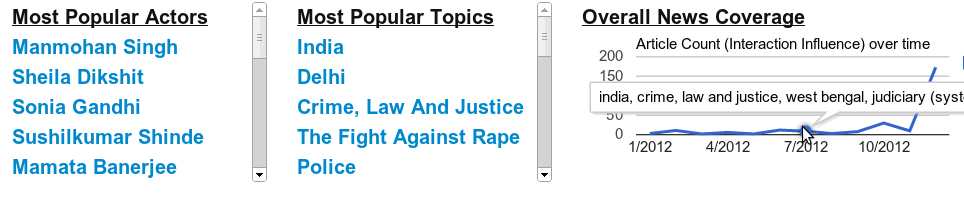
\includegraphics[width=9cm,scale=0.30]{figures/faceted2.png}
\label{fig:faceted-search}
\end{center}
\end{figure}

\subsubsection{Structured storage of an article stream}
The rate at which new articles are published is growing exponentially. If a system
has to do well at taking in a live input stream of news articles, it can afford to process this set only once, and then store this set in a structure
which is efficient to maintain and query later. Since our back-end is a graph, we can efficiently query looking only at the graph metadata. 
Moreover, if the articles are coming from a third-party, they need not be stored at our server (once we build the graph), we can query them on-demand. 

\subsubsection{On-demand detail}
The system should respect the user's final say in the detail at which different stories are visualized. Should the system
just give a 10-line summary of the event captured by 5 articles? Or should it focus in to the 5 articles, creating 2 sub-stories within them? This decision
should be left to the user as a preference.

\subsubsection{Summarizing News stories}
We summarize news articles constituting a particular news story to make it easy for a user to the gist of the story. This helps the user to quickly decide whether the story interests her or not.

\subsection{System Overview}
\label{sec:block}

Figure~\ref{fig:block-system-design} presents our system architecture. It can be divided into
two major components - Offline and Online. The offline component handles incoming news articles, and augments them into our underlying graph data structure representation stored
in the database. The online component interfaces with the user, and based on the user's query, identifies the parts of the graph to visualize and 
shows the relevant stories. We will now briefly describe each aspect of our system.

\subsubsection*{News Corpus}
Our news corpus is a subset of articles from the Indian national daily {\em The Hindu}\footnote{http://thehindu.com}, across a variety of broad categories like Crime, Economy, Government, etc. 
{\em The Hindu} was chosen because it is a popular Indian daily, and offers a convenient way to download articles along with rich meta-data like Topic tags.

\subsubsection*{Entity Extraction}
We used the OpenCalais\footnote{http://opencalais.com} API to extract all the entities appearing in the articles. In particular, we call
the people featured in the articles as actors. We found the result of OpenCalais to be the most accurate among the NER tools we experimented with.
For sanitizing the mined entity set (correct spelling errors, remap aliases of the same entity to a unique identifier, remove ambiguous entity tokens),
we used an ontology(YAGO\footnote{http://www.mpi-inf.mpg.de/yago-naga/yago/}) based approach.

\subsubsection*{Topic Detection}
Along with the entities for an article, we also need the list of topics that were talked about in the article. 
We relied on the Hindu articles being hand tagged-at-source by rich and relevant Topic tags. These are much more expressive compared to an automated technique of topic detection.
\begin{figure}
\caption{Block system diagram of our News Browsing tool}
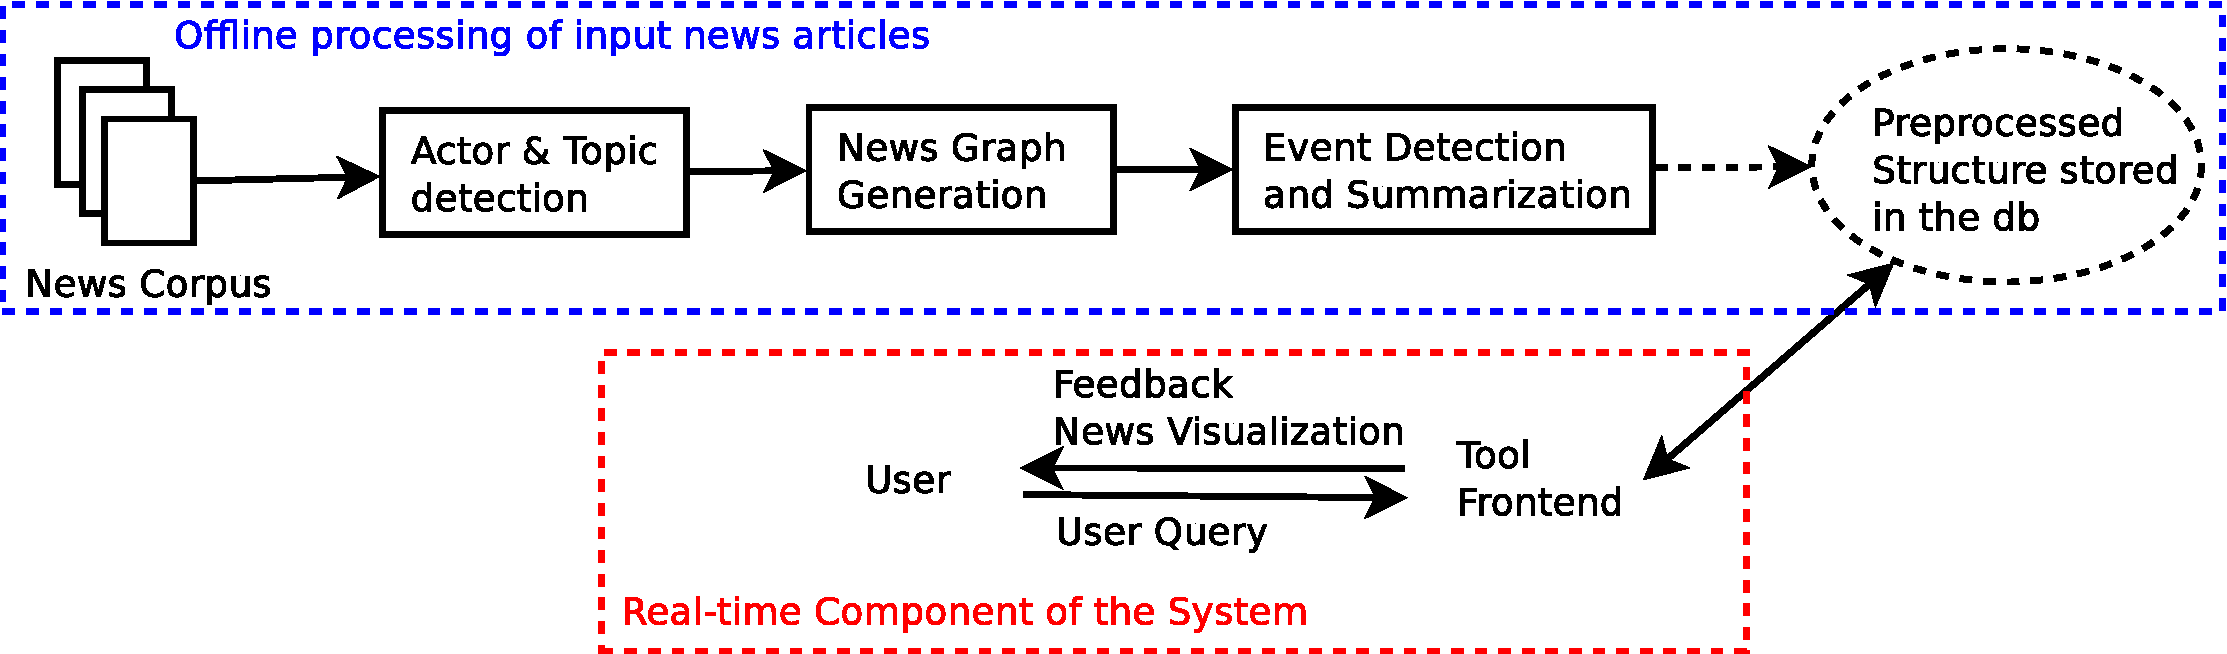
\includegraphics[scale=0.24]{figures/system-design.pdf}
\label{fig:block-system-design}
\end{figure}

\subsubsection*{News Graph Generation}\label{sec:graph-desc}
We follow the same graph geenration algorithm described in Choudhary et al.\cite{choudhary@ecir2008}. We extended their algorithm to
augment new articles as they are published on to the graph built up to that time. The following sequence of update steps are to
be followed on augmenting a new article $a$ published at $\tau$, into the graph structure.
\begin{enumerate}
  \item Preprocess $a$ to mine relevant actors and topics
  \item For all articles $b \in \mathcal{A}[\tau - P, \tau]$
  \begin{itemize}
  \item Mine and score all transformations between the articles $a$ and $b$
  \end{itemize}
  \item Find an edge-covering of the new transformations connecting node $a$ to nodes in $\mathcal{A}[\tau - P, \tau]$
\end{enumerate}

By taking the recommended values of the parameters($F=50$ days, $P=50$ days), we were able to generate a news graph on 1000 nodes in around 4 minutes on a Dell Intel Centrino machine.
Adding newer articles to this graph was significantly cheaper, taking only around 10 seconds depending on the article size, etc.
Moreover, it only looks at articles within a time window, and hence different parts of the graph can be generated in parallel.

\subsubsection*{Event detection}
\label{sec:event-detection-summary-context}
The news graph created is clustered with a standard graph clustering algorithm: Markov graph clustering \cite{Dongen00a}.
We used the Article similarity $r(a,b)$ as defined in \ref{subsec:article_similarity} as the flow (transition probability) from a node $a$ to $b$ by normalizing $r$ to get the quantity $r_n(a, b) = \frac{r(a, b)}{\sum_{b \in N(a)}r(a, b)}$. We can now formulate the flow matrix using these scores and run the Markov Clustering Algorithm. We used the standard inflation factor of 2 as our input for forming the clusters. 

As we show in Section~\ref{sec:baseline-comparison}, events determined by way of clustering on the graph are preferred by users to a similar TfIdf text clustering done on raw articles in most cases.

\subsubsection*{Event summarization}
To make it easier for the user to understand an event, we summarize the articles of this event to give a broad idea of the event and show this summarization alongside the articles capturing that event (Section \ref{sec:filter-summarization}). For this, we tried out various document summarizing tools. We finally decided to Text Compactor \footnote{http://textcompactor.com/} which is based on Open Text Summarizer\footnote{http:/libots.sourceforge.net/} and has a convenient API. 
\begin{figure*}[ht]
\caption{A screenshot of our tool visualizing Rape-related cases from India in 2012}
\center{
    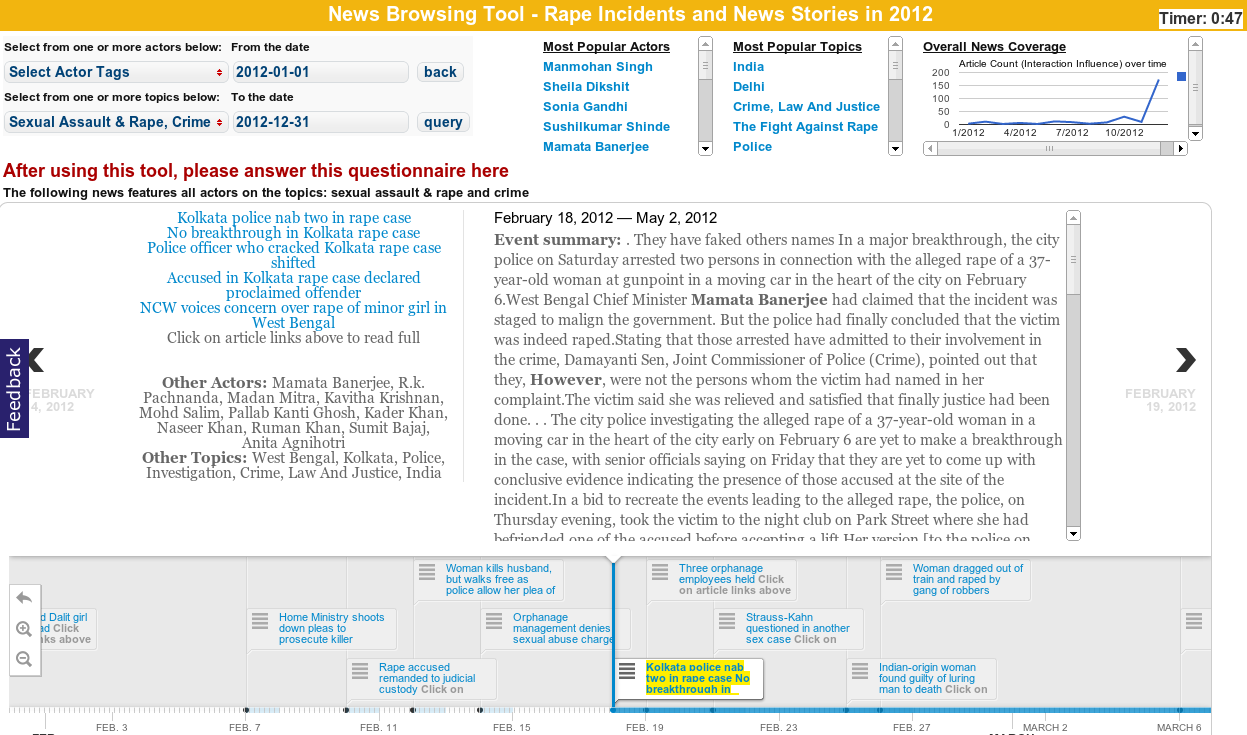
\includegraphics[scale=0.3]{figures/complete.png}
}
\label{fig:complete-tool-screenshot}
\end{figure*}
\subsection {Frontend interface}
Our interface is built on HTML using Javascript and PHP on the server-side, using TimelineJS\footnote{http://timeline.verite.co/} and Google Visualization API\footnote{http://developers.google.com/chart/interactive/docs/reference} libraries.
Figure~\ref{fig:complete-tool-screenshot} shows a screenshot of our webtool. The interface
has 3 primary parts: the Filtering \& feedback pane, the News article(s) \& summary pane and the Timeline pane. 
\subsubsection*{Filtering \& feedback pane}
Our system deeply analyzes the news corpus to mine all the featured actors and topics, and makes them queryable. The user selects one or more actors
and/or topics to filter news only about them. The user could also restrict on a particular time window. Relative to the filter parameters set by her, 
the user gets more context by way of getting a ranked list of ``Popular Actors'' and ``Popular Topics''. In addition, we also plot the number of
articles published against time to study what stories were popular at what times. 
 
\subsubsection*{News articles \& summary pane}\label{sec:filter-summarization}
Having selected a particular story to focus on, the user can read all articles arranged sequentially so it is easy to read them in succession.
On the right, we show a summary generated from the articles of this story by the methods discussed in Section \ref{sec:event-detection-summary-context}.
On clicking an article, the user is served the full article text. The user is also shown the full list of actors and topics discussed in this story.
\subsubsection*{Timeline pane}
Having selected suitable filters, the user is presented with all the different events detected from the graph on the timeline. These appear as 
bubbles on the timeline, with a start and end date. The user can easily move in time, skimming through uninteresting news events.
More popular events (as judged by the density of nodes \& edges in the cluster), are highlighted in yellow to guide the user.
On clicking a particular bubble, that event is highlighted and the corresponding story is shown in the middle pane.
